\chapter[Conclusions and Future Work]{Conclusion and Future Work}
\chaptermark{Conclusions and Future Work}
\label{chap:conclusion}
\minitoc

\newpage

In this section, we will highlight some of the major contributions that were achieved within this thesis. We will further discuss the major shortcomings as well as future prospectives that could address those limitations. 

\section{Summary}
In the introductory \chapref{chap:introduction}, we analyzed the inevitable rise of robot assisted laparoscopy and linked it to surgeon benefits and future prospects, \secref{in:sec:the_rise_of_robot_assisted_laparoscopy}. We identified spatial awareness and automation as key targets for enhancing and alleviating, driving factors and roadblocks, respectively, see \figref{in:fig:advancing_robotic_laparoscopy}. To address these, we proposed marker-free unified calibration for enhanced spatial awareness with improved clinical workflow in \secref{in:sec:marker_free_unified_calibration}. Moreover, in \figref{in:fig:hypothesized_pipeline}, we outlined a framework for learning to imitate camera motion from a camera-assistant-held laparoscope, see \figref{in:fig:room_setup}. We argued that, through a mixture of classical control, and imitation learning in image space, it might be possible to imitate a surgeon through a robot laparoscope holder despite their different embodiment. The following sections will discuss the extend to which the proposed solutions met the pinpointed targets, and further suggest future research directions when targets where not fully met or could be improved upon.

\section{Marker-free Unified Eye-hand Calibration}
\label{con:sec:marker_free}
\paragraph{Contributions} In \chapref{chap:registration}, we introduce a novel marker-free unified eye-hand calibration procedure. The method solely relies on stereo RGB-D images, robot mesh or CAD files, and joint position readings, see \figref{c1:fig:hydra_registration}. We contribute an algorithm for robust point-to-plane \acrshort{icp} in \algoref{c1:alg:liep2plan}. Extensive comparisons of single-shot capabilities against classical eye-in- and eye-to-hand as well as handshake calibrations are demonstrated on system, see \figref{c1:fig:calibrations}, and on-par results are summarized in \tabref{c1:tab:calibration_results} with visually good alignments in \figref{c1:fig:registration_results}. We finally deploy an improved version of the method in a clinically relevant scenario, \figref{c1:fig:in_vivo_setup}, and showcase qualitatively accurate renders in \figref{c1:fig:in_vivo_results}, with close to perfect IoUs in \tabref{c1:tab:iou}, and corresponding minor segmentation-render differences in \figref{c1:fig:masks}.

\paragraph{Shortcomings and Future Work}
\begin{figure}[tb]
    \centering
    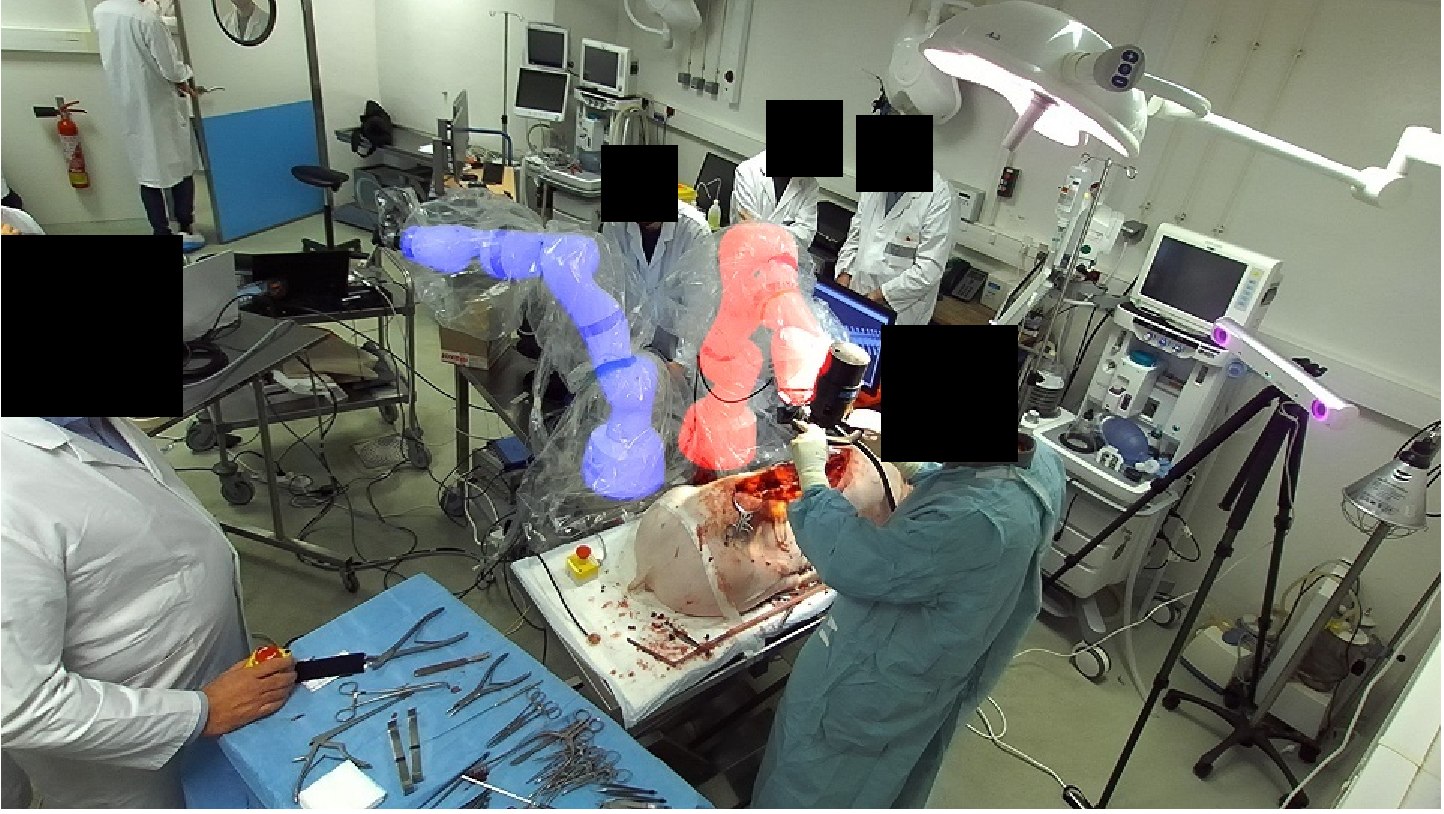
\includegraphics[width=\textwidth]{conclusion/img/draped_ground_truth.pdf}
    \caption{Render of robots, given the registration results of \secref{c1:sec:in_vivo_results}, overlayed on view in draped stage. Hyperspectral camera robot (left, blue) and drilling robot (right, red), see \figref{c1:fig:in_vivo_setup}. Refers to \secref{con:sec:marker_free}.}
    \label{con:fig:draped_ground_truth}
\end{figure}
The proposed robust \acrshort{icp} already exhibits convincing registration results and impressive scalability to any industrial serial manipulator with, compared to the differentiable rendering alternatives, little dependencies. In the clinical context, however, draping poses a procedural necessity that renders the proposed approach infeasible. As such, future work should focus on marker-free registration despite draping. To this end, we contribute a dataset of draped robots with ground-truth registrations, see \figref{con:fig:draped_ground_truth}.

\paragraph{Key Takeaways}
In \chapref{chap:registration}, we address the need for improved spatial awareness with unaltered clinical workflows, \secref{in:sec:spatial_awareness}, \figref{in:fig:advancing_robotic_laparoscopy}. We contribute a novel dataset for first steps towards clinical translation on draped systems. Moving forward, this research should enhance modular systems \secref{in:sec:robot_surgery_platforms}, \tabref{in:tab:systems}, with accompanying benefits such as reduced cost and operation time. Serial manipulators in industrial applications could benefit through the presented approach immediately.

\section[Homography-based Visual Servo with \acrshort{rcm}]{Homography-based Visual Servo with Remote Center of Motion Constraint}
\label{con:sec:visual_servo}
\paragraph{Contributions} In \chapref{chap:robotic_endoscope}, we introduced a novel image-based visual servoing approach with \acrshort{rcm} constraint. We attempted to shift the control paradigm from a tool-centric control policy towards a view-centric control policy to address the flaws of the dominant visual servos, refer \secref{in:sec:rule_based_approaches}, \figref{in:fig:com}. To this end, we derived a homography-based visual servo which does not rely on depth nor on tool distance for inferring actions \figref{c2:fig:schematic}. We did so, introducing a projection operator for mapping target camera frame velocities to available DOF, \eqref{c2:eq:proj}. We then deployed the newly derived control in a novel view-graph-based semi-autonomous scheme on a real system, see \figref{c2:fig:pipe}, \figref{in:fig:experimental_setup}. The proposed method demonstrated good image space convergence properties throughout traversing the view graph from current to target view whilst retained a deviation from the target \acrshort{rcm} below $5\,\text{mm}$, see \figref{c2:fig:errors}. The proposed method further indicated robustness against patient re-positioning, i.e. coordinate system change, see \tabref{c2:tab:repositioning}.

\paragraph{Shortcomings and Future Work} The most apparent shortcoming of the proposed method is the assumption of a mostly static surgical scene which clearly does not hold, see \figref{c2:fig:tool_insertion_trajectory}. This temporality assumption, however, is not so crucial within the overarching context of the thesis, as ultimately the executed action is not graph-based but rather incrementally sampled from a learned expert policy $\pi_\text{E}:\, \hat{s}_t \rightarrow \hat{a}^*_t$, refer \secref{in:sec:imitation_learning}. A shortcoming that weighs much heavier is e.g. the lack of force sensing. No trocar-laparoscope external forces nor arm-environment external forces are incorporated into the controller. Arm-environment external forces could e.g. be minimized through nullspace projection and the redundant DOF of the manipulator. The proposed controller furthermore does not explicitly constrain solutions to the \acrshort{rcm}, and convergence to undesired minima might occur. Further research should thus introduce constrained optimization instead.

\paragraph{Key Takeaways} Altogether, it was demonstrated that indeed the introduced visual servo could serve as means for executing actions $\hat{a}^*_t$ for the hypothesized pipeline, refer \figref{in:fig:hypothesized_pipeline}, but that future improvements would be necessary for successful clinical translation.

\section{Homography-based Camera Motion Estimation}
\label{con:sec:hom_est}
\paragraph{Contributions} In \chapref{chap:camera_motion_extraction}, we introduce a novel data augmentation \algoref{c3:alg:hom} for runtime generation of synthethic camera motion, see \figref{c3:fig:hom}. We introduce a new dataset of camera motion separated da Vinci\textsuperscript{\textregistered} surgery image sequences through exploitation of the clamping mechanism, which we initially proposed in \figref{in:fig:camera_motion}. Therefore, we utilize all available high frame rate datasets from \tabref{in:sec:search_for_available_data} and summarize their respective sizes in \figref{c3:fig:data}. We conduct an extensive backbone search for models that are regressed onto the synthetic data across multiple compute regimes and devices, \tabref{c3:tab::results}. For evaluating the transferability from videos of \acrshort{rmis} to \acrshort{mis}, we hand-annotate static landmarks in video sequences of laparoscopic interventions \figref{c3:fig:seg}. We find that models which are supervisedly trained on the novel dataset with the novel \textit{homography generation algorithm} outperform classical feature-based homography estimators. We find that they only outperform classical methods when trained on sequence lengths $N>1$, see \figref{c3:fig:resnet34}, justifying our proposed approach. We further find that the learned models outperform the feature-based ones across varying edge deviations $\varrho$. A quantitative statistical significance is shown in \figref{c3:fig:resnet34_c}. Qualitatively we find that static vessels in the background are aligned better through our novel approach, \figref{c3:fig:qualitative}.

\paragraph{Shortcomings and Future Work}
\begin{figure}[tb]
    \centering
    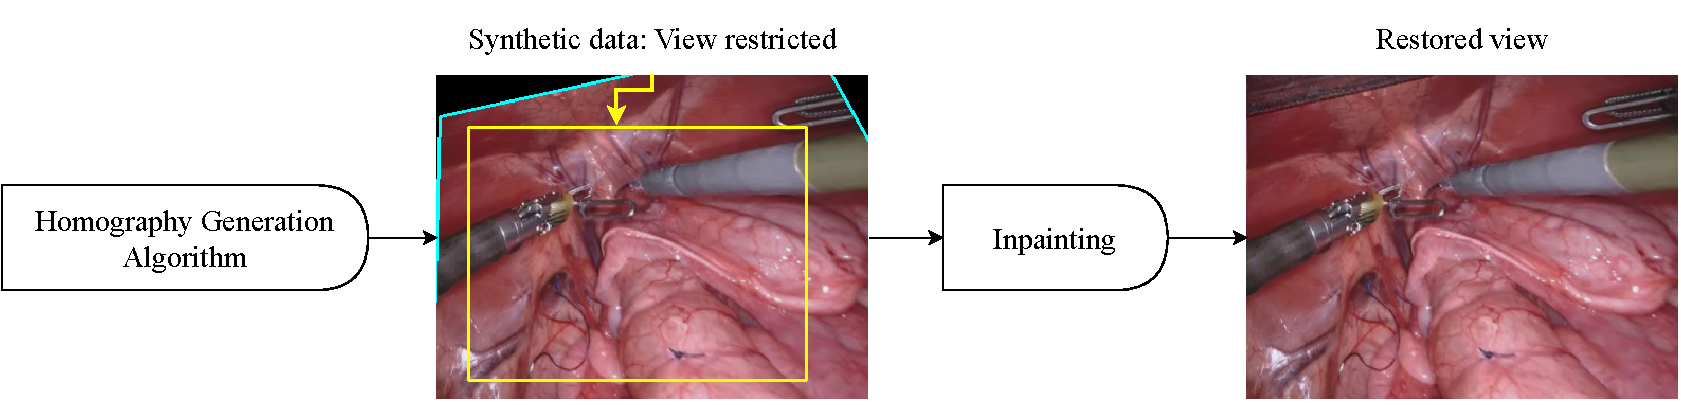
\includegraphics[width=\textwidth]{conclusion/fig/fourier_inpainting.pdf}
    \caption{Proposed inpainting for data retrieval. The \textit{homography generation algorithm} from \secref{c3:sec:hom_gen}, \figref{c3:fig:hom}, introduces black boundaries and thus restricted views. Generative inpainting could help restore the entire view. Fourier inpainting done via~\cite{suvorov2021resolution}, \textbf{not} fine-tuned. Refers to \secref{con:sec:hom_est}.}
    \label{con:fig:inpainting}
\end{figure}
Whilst significant improvements are demonstrated over state of the art homography estimates, there still exist shortcomings of this work. The \textit{homography generation algorithm}, although capable of generating indefinite synthetic camera motion, introduces the necessity to crop the view as otherwise black borders would be introduced. This intrinsically limits the magnitude of synthetic camera motion and therefore also the range of learnable camera motion. This fact is somewhat underevaluated through the hand-annotations from \figref{c3:fig:seg} as images were annotated on a frame-to-frame basis with relatively little camera motion in-between. For future work, we suggest to train a generative inpainting model that restores the entire view post camera motion generation, see \figref{con:fig:inpainting}. In this example, an unrefined inpainting model was utilized, showcasing the feasibility of dedicated methods. We suggest the use of a standard generative approach as opposed to diffusion models, such as~\cite{rombach2022high}, since the iterative process might not satisfy the runtime requirements of the \textit{homography generation algorithm}. Furthermore, future research might aim at incorporating depth information for camera motion synthesis, e.g. through~\cite{budd2024transferring}.

\paragraph{Key Takeaways} \chapref{chap:camera_motion_extraction} introduced several novelties for estimating camera motion in dynamic surgical scenes despite the presence of tool and organ motion, proving the hypothesized pipeline in \figref{in:fig:camera_motion}. As such, the work presented in~\cite{huber2022deep} presents the state of the art methodology for generation of state-action pairs $(\hat{s}_t, \hat{a}^*_t)$, refer \secref{in:sec:imitation_learning}, to be used in the imitation learning proposal of \figref{in:fig:hypothesized_pipeline}.

\section{Homography-based Camera Motion Prediction}
\label{con:sec:hom_pred}
\paragraph{Contributions} In \chapref{chap:camera_motion_prediction}, we introduce a novel approach for fully self-supervised camera motion imitation learning from retrospective videos of laparoscopic surgeries, refer \figref{c4:fig:training_pipeline}. The proposed method utilizes the camera motion extraction of \chapref{chap:camera_motion_extraction} to generate state-action pairs at runtime, for which efficiency is demonstrated in \tabref{c4:tab:estimation_speed}. This approach allows us to introduce the separation of photometric and geometric transforms, such that behaviors can be learned regardless of the relative patient positioning, as we can still extract camera motion on geometrically transformed sequences. The proposed method leverages a novel importance sampling, which is grounded on an analysis of camera motion distribution over large-scale video datasets of cholecystectomies, see \figref{c4:fig:camera_motion_distribution}. Without this importance sampling, only identity policies would be learned. We then contribute the first large-scale imitation learning on publicly available data and find significantly improved performance over baselines \tabref{c4:tab:camera_motion_prediction}. We reaffirm this finding through predicting camera motion on the AutoLaparo dataset~\cite{wang2022autolaparo}, and showcase that the predicted motion aligns with the provided labels \figref{c4:fig:autolapato_results}. A qualitative prediction on a video sequence is shown in \tabref{c4:tab:camera_motion_prediction}.

\paragraph{Shortcomings and Future Work}
While this work demonstrates that camera motion can be predicted in a fully self-supervised manner, it does still have shortcomings. One of the major shortcomings that were not addressed is the limited preview horizon $M=1$, see \secref{c4:sec:model_architecture}. As such, the model only predicts $0.25\,\text{s}$ in advance and could, e.g. not be used for model predictive control. It further only has a context window, i.e. the recall horizon, of $N=14$ or $3.5\,\text{s}$. For increased context window sizes, it might be crucial that the camera motion estimator, \figref{c4:fig:training_pipeline}, is capable of estimating larger motions, which is an inherited issue of \secref{con:sec:hom_est}, and could be addressed through \figref{con:fig:inpainting}. The model is thus mostly suited for predicting how motion will continue but currently lacks bootstrapping capabilities. Part of the reason for lacking bootstrapping capabilities can further be found in the partial state observance, see \figref{in:fig:hypothesized_pipeline}. The proposed method only accesses iamges $\hat{s}_t$, and does not have any prior procedural knowledge, which we argued was beyond scope of this thesis, nor knows about device readings or surroundings in general, which are inaccessible in the public datasets. However, with the advent of massively pre-trained large language models, such as Llama~\cite{touvron2023llama}, Mistral~\cite{jiang2023mistral}, and GPT-4~\cite{achiam2023gpt}, the incorporation of procedureal knowledge might become feasible, as can already be observed in tasks such as visual question answering~\cite{seenivasan2022surgical}. Ultimately, this might lead to foundation-like models for laparoscopic camera motion action prediction. For these types of models, although we discarded simulation-based \acrshort{rl} in \secref{in:sec:reinforcement_learning}, \acrfull{rlhf} might become a relevant research direction, which is much more sample efficient than pure \acrshort{rl}. Admittance controllers with \acrshort{rcm} which are suitable for \acrshort{rlhf}, can e.g. be found in \appref{app:lbr_stack}.

\paragraph{Key Takeaways}
In \chapref{chap:camera_motion_prediction}, we found first indicators that actions $\hat{a}^*_t$ might indeed be immediately learnable tasks, similar to the auxiliary tasks from \figref{in:fig:auxiliary_tasks}. We thus closed the loop for the hypothesized pipeline of \figref{in:fig:hypothesized_pipeline}, but argued that further research would be necessary.

\section{Closing Remarks}
%In this thesis, \textit{Data-driven Robotic Endoscope Automation}, we outlined to address level five autonomy in the Foreword \secref{in:sec:foreword}. Following a comprehensive review of relevant domains, from clinical, economic, and technical perspectives, we drafted a general approach to embodiment-invariant imitation learning from observation in \figref{in:fig:hypothesized_pipeline}, \secref{in:sec:hypothesizing}. We instantiated this proposed method through novel and innovative solutions, and discussed contributions, as well as shortcomings for each building block from \secref{con:sec:marker_free} to \secref{con:sec:hom_pred}. We wish to emphasize that level five autonomy has not been achieved, but that major steps towards it were taken. Exciting new research directions were discovered and new opportunities were created. In fact, this thesis creates more questions than it answered, and we hope that future research can build on top of it.

In this thesis, titled \textit{Data-driven Robotic Endoscope Automation}, we embarked on a journey to address level five autonomy as introduced in the Foreword (\secref{in:sec:foreword}). Through a thorough exploration of various domains—clinical, economic, and technical—we formulated a holistic approach to embodiment-invariant imitation learning from observation, illustrated in \figref{in:fig:hypothesized_pipeline} (\secref{in:sec:hypothesizing}). Implementing this conceptual framework led to the development of novel solutions discussed in detail across sections from \secref{con:sec:marker_free} to \secref{con:sec:hom_pred}. It's important to note that while level five autonomy remains elusive, significant strides have been made. This work not only sheds light on promising avenues for future research but also underscores the emergence of new challenges and opportunities.

In the spirit of fostering a beginner's mindset, we conclude with a quote from the book Zen Mind, Beginner's Mind:

%In the hope, that this thesis forms a beginners perspective, I would thus like to end it with a quote from the book Zen Mind, Beginner's Mind, and hope this thesis is far from :

\topskip0pt
\vspace*{\fill}
\begin{center}
\textit{In the beginner’s mind there are many possibilities, but in the expert’s there are few.}

\vspace{5mm}
\hspace{20mm} --- Shunryu Suzuki~\cite{beginnersmind}
\end{center}
\vspace*{\fill}

As such, we envision this thesis serving as a catalyst, fostering innovation and inspiring fresh perspectives in approaching this complex problem of laparoscopic camera motion automation.


%\begin{itemize}
%    \item general pipeline for imitation learning ..... with clinically safe application
%    \item the general pipeline might be investigated through several means in the future...
    %the proposed pipeline holds an interesting framework for self-supervised .... indeed proving that \figref{in:fig:auxiliary_tasks}
%    \item innovative and novel ways
%    \item found exciting research directions and created opportunities
%\end{itemize}
